\documentclass[letter, 11pt]{article}
\usepackage{comment}
\usepackage{fullpage}
\usepackage{graphicx}
\begin{document}

\noindent
\begin{center}
\large\textbf{Apotheosis} \\
\textbf{A Spotify Aggregation Site}
\end{center}

\noindent
\normalsize CSE321 - Web Programming\\
\textbf{Group 5:} The Wonderous Avacados\\
Sterling Blevins, Damon Estrada, Sarah Masters\hfill September 5th, 2019
% NOTE: Names are alphabetical by last name
 
\section*{Background}
The group has decided on designing a website that utilizes the Spotify API because of interest in data analytics, presentation, and the application of a widely available and common API into a project. The Spotify API is a very functional and powerful tool which will allow us to process music for each individual user of the service. We will be able to demonstrate out knowledge of web programming tools while possibly contributing a useful and interactive tool for music listeners everywhere. 

\section*{Website Analysis}

\noindent
\textbf{Musical Data Functions{\textsuperscript{[1]}}:}\\
This website provides statistical information on individual songs. It uses a spider graph to show the user various parameters of a song (valence, dancability, etc). In addition, it offers insight on the popular tracks from the artist in a region selected by the user and statistics on the artist.
\setlength{\parskip}{7pt}

\noindent
\textbf{Playlist Manager Functions{\textsuperscript{[2]}}:}\\
This website allows a user to merge a lot of songs together from multiple playlists. This creates one view which allows the user to modify their existing playlist opposed to changing playlists one at a time. This can be helpful especially when the user has a lot of playlist to manage or if they have a lot of playlist.
\setlength{\parskip}{7pt}

\noindent
\textbf{Music Popcorn Functions{\textsuperscript{[3]}}:}\\
This website visualizes genres to the user. Essentially, it clumps genres and sub-genres together alike while distancing the opposite genre as far away as possible visually. This helps show the more important genres being bigger and unknown or less popular genres smaller (popcorn). The user can then explore these genres by clicking on them and being shown songs and artist labeled under each genre.
\setlength{\parskip}{7pt}

\noindent
\textbf{Discover Quickly Functions{\textsuperscript{[4]}}:}\\
This website brings an interface for the user to listen to tracks in a fast manner. Users are usually interested or not in a song within the first few seconds. The website allows the user to hover their mouse over a track while it plays at a key moment in the track to allow the user to decide if they like tit or not. This allows the user to quickly shuffle through recommendations, tracks, and even playlist quickly if under a time constraint or simply trying to find a new song fast.
\setlength{\parskip}{7pt}

\noindent
\textbf{Replayify Functions{\textsuperscript{[5]}}:}\\
This website while basic is informational. It shows the user their latest songs played based on a time period Spotify keep track of in their API. They have short (within the month), medium (past 6 months), and long (last year to the beginning of time) term tracking. This website utilizes to show the user their most played songs respectively to the time period chosen.
\setlength{\parskip}{7pt}


\noindent
\textbf{Analysis Summary:}\\
The group would like to implement a blend of the mentioned websites similar to our theme. Ideally, we would like to gain as much information on the user as possible through their inputted preferences and data already collected on them. We would use this information to construct personalized playlist for them that differ from the ones already constructed through Spotify. Also, we would like to offer track suggestions based on current listening and other events that the user might be performing at the moment. In addition, we would like to offer statistics to the user based on their listening habits to have them gain insight on their habits or interesting facts about themselves. Finally, we would like to display all of this data in a clean and efficient manner while trying to make it interactive and interesting for the user.
\setlength{\parskip}{7pt}

\noindent
\textbf{Functionality Comparison Table:}\\

\noindent
\begin{tabular}{ |p{3cm}|p{2cm}|p{2cm}|p{2cm}|p{2cm}|p{2cm}|p{2cm}|  }
 \hline
 Function & Proposed System & Musical Data \textsuperscript{[1]} & Playlist Manager \textsuperscript{[2]} & Music Popcorn \textsuperscript{[3]} & Discover Quickly
 \textsuperscript{[4]} & Replayify
 \textsuperscript{[5]}\\
 \hline
 Service Login & V & X & V & X & V & V\\
 Playlist Creation & V & V & X & X & X & V\\
 Suggestions & V & V & V & V & V & X\\
 Statistics & V & V & O & V & O & V\\
 Data Display & V & V & O & V & O & V\\
 Interactive & V & V & V & V & V & V\\
 Data Export & V & X & X & X & X & X\\
 \hline
\end{tabular}

\textbf{KEY:}\\
\indent
V: Able to perform the task \\
\indent
X: Unable to perform the task \\
\indent
O: Able to perform the task with poor interactive design

\section*{Users of the Website}
\noindent
\textbf{Spotify Listeners:}\\
The users of the Spotify Music streaming service would be one of the users of our site. We will offer the ability to add new playlists based on listening preferences. In addition, we can show information related to the user's music listening habits which could lead to the discovery of new music or artists as suggested by our site.

\noindent
\textbf{Non-Spotify Listeners:}\\
The non users of the Spotify Music streaming service could also be a user of the site. They will not get customized settings and listening preference suggestions, but can still look at the visualization of the most popular music of the current day. The user will be able to look at what is available and see if the site service would be worth creating an account.

\section*{Desktop Version of Site}

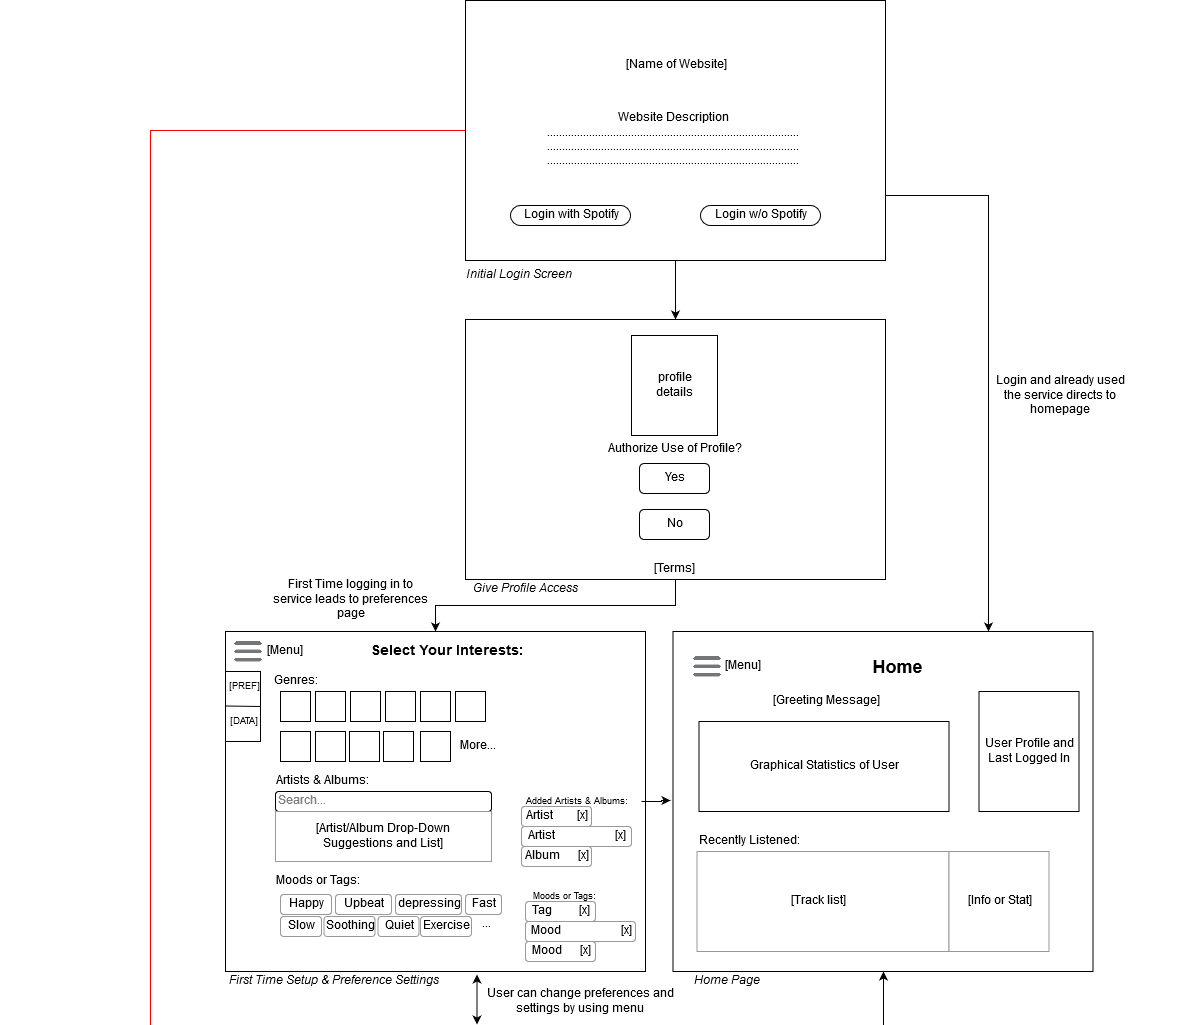
\includegraphics[scale=0.57,left]{storyboard_1.png}\\
For the above figure, it represents the login screen in addition having an option to not sign in with Spotify. Members who are registered with Spotify will benefit greatly if they are with our website since the will be given tailored recommendations and statistics directed towards them rather than an audience. With that in mind, non-members will be shown demographics based on region and other factors that will only show vague statistics rather than specific ones.\\
After the login screen, another screen (if a registered member of Spotify) will display to gain authorization from the user to utilize their data. After this, one first visit to the website the user will be prompted with various filters on their interests in music such as genres, artists, track features, and more. From this, the user will then be directed towards the home screen while if a non member logged in, they would skip the mentioned screens and go straight towards the home screen.\\
A registered member at any time can change their preferences in the preference settings menu while a non-member cannot. The Home page will show the previously mentioned statistics to a member and vague statistics towards a non-member.\\

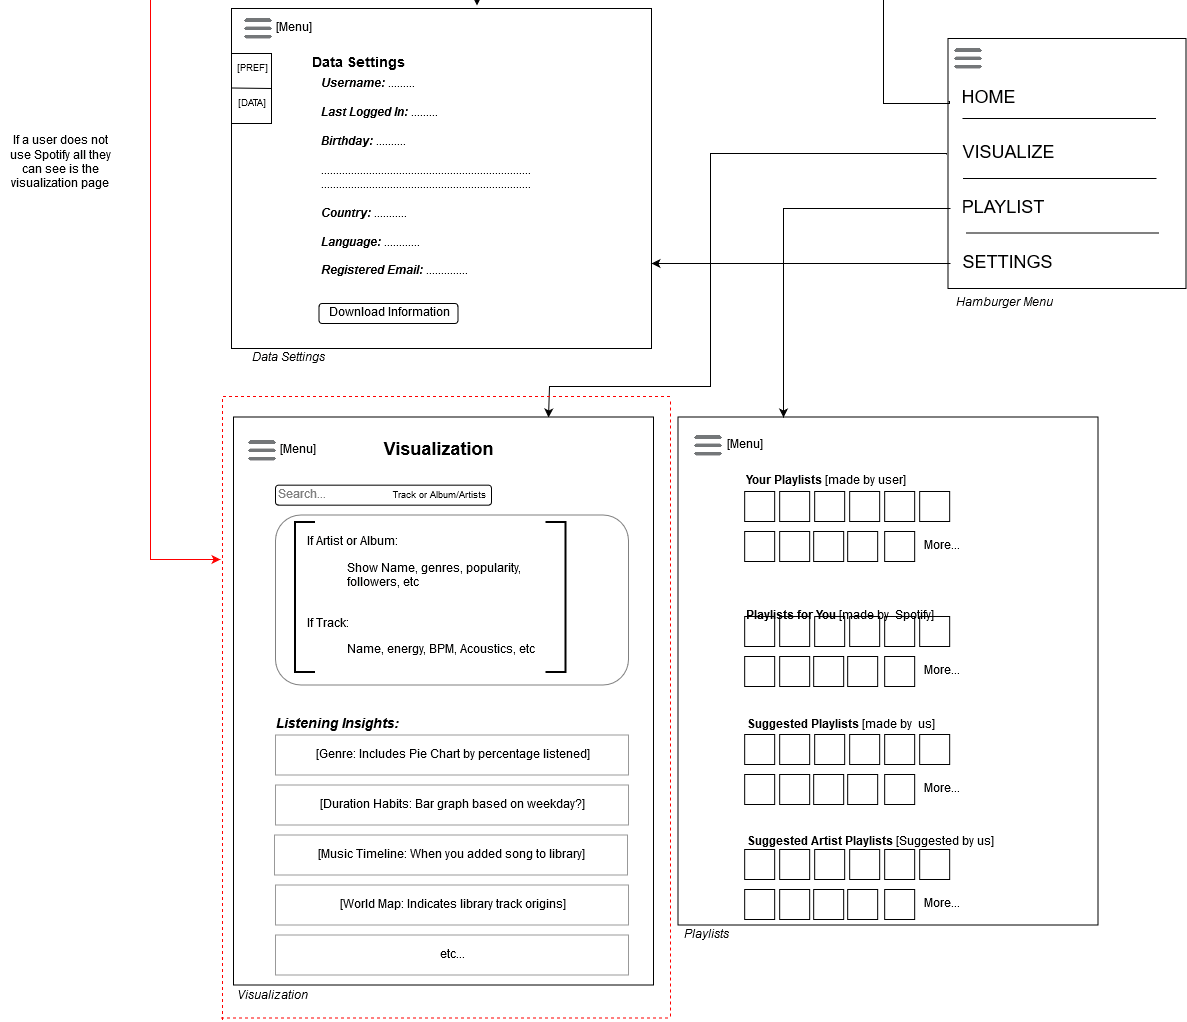
\includegraphics[scale=0.57,left]{storyboard_2.png}
The above figure is a continuation of the introduction of the website. At anytime if a user clicks on the menu icon shown as three horizontal lines, a slide out menu shall appear which will prompt the user of the various tabs or pages that the website supports or can navigate to. This will include the home, visualization, playlists, etc screens. The visualization screen will show graphical representations of the statistics collected by a member and for a non-member will be shown graphs, charts, or other graphs of non-member related statistics. Upon navigating towards the playlist screen, the user (member) will be prompted with our hand picked playlist that we feel the user will like based on their preferences and likes while a non-member will be shown what is popular in their region.\\
The great thing about the flow or navigation between pages is the ability to go between each without meeting specific conditions. Meaning that the home screen can navigate to any pages and so can the others.\\

\section*{Mobile Version of Site}\\

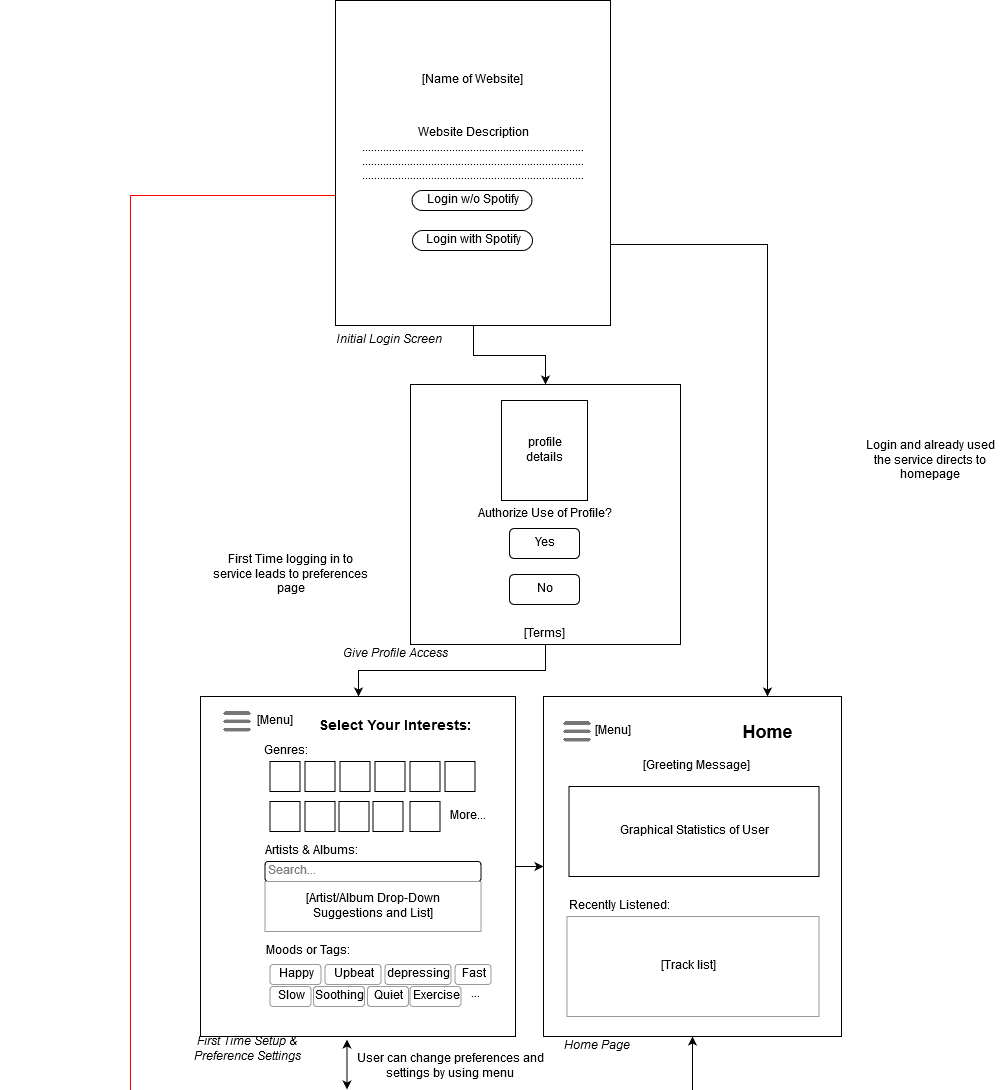
\includegraphics[scale=0.57,left]{storyboard_1_mobile.png} \\

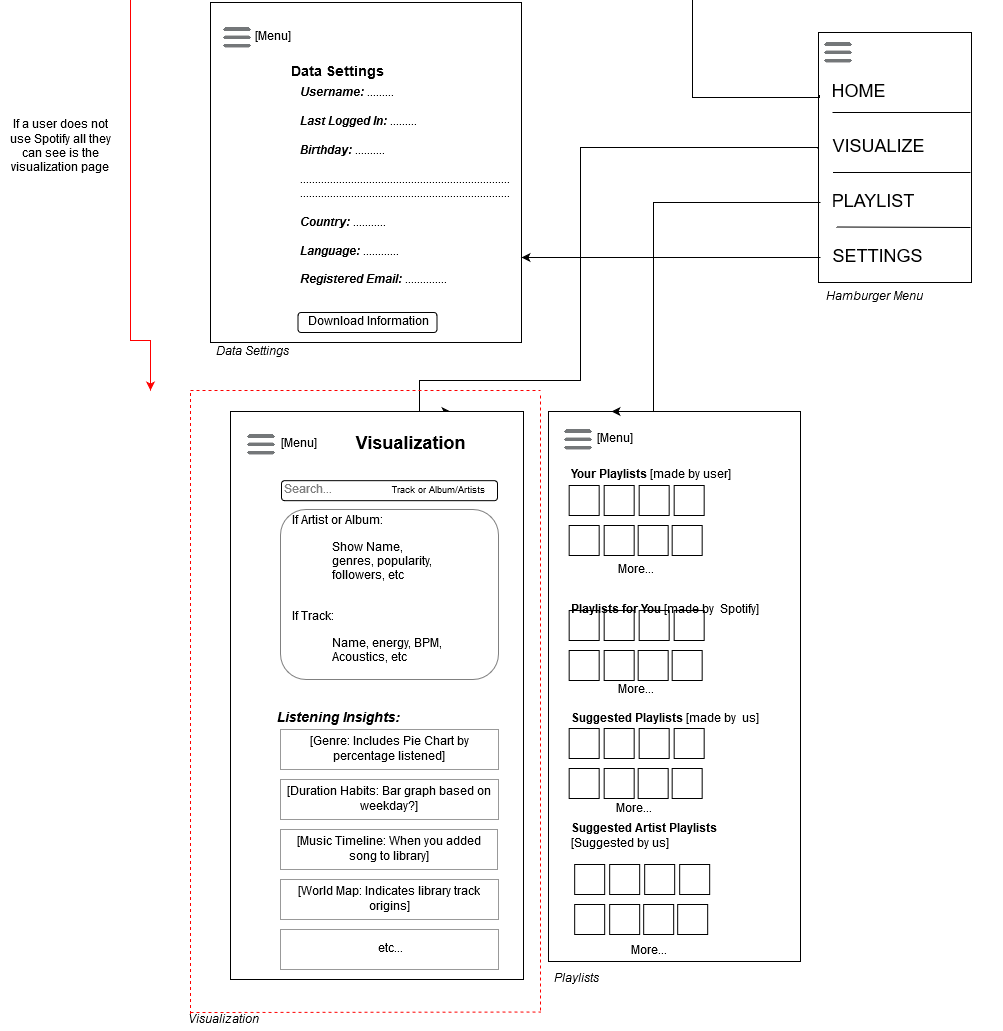
\includegraphics[scale=0.57,left]{storyboard_2_mobile.png}\\
For the mobile version, the exact layout is followed from the website version. The only constraint is screen size so we will have to refactor the graphical representation of the site. This means and pictured below that some things will be reduced in size to accommodate the size of the screen but will still supply the same things the website does in a longer scrolling manner that the user will have to perform (scroll down more so).\\
\\
\\

\section*{ER Diagram}

The purpose of this section is to demonstrate the layout and plans for the website's database. This involves a diagram of the schema, an ER diagram involving the tables, and an explanation of the contents of the tables.

\section*{ER Schema}

\includegraphics[scale=0.46,left]{ER_schema.png}

The ER schema behaves as a guideline for the relationships between the entities and and all of the attributes related to these entities. For our website, the general idea is the user is identified via a unique User ID, a name, language, etc. The user has preferences made up of moods and genres. The user also has playlists from either Spotify or generated by us: each identified by their own ID, containing tracks, etc.

\section*{ER Diagram Tables}

\includegraphics[scale=0.65,left]{ER_tables.png}

The ER Table shows the actual table entities, and the relationship between the tables. Each attribute behaves as a column, and each unique identifier (underlined in the schema above) is denoted with a key. The attribute that the key connects to in another table, represents a foreign key, indicating that the tables are related and overlap content.

\pagebreak

\section*{Database Table Descriptions}

The tables below show the contents of the tables, primary keys, data types, foreign keys, and comments.

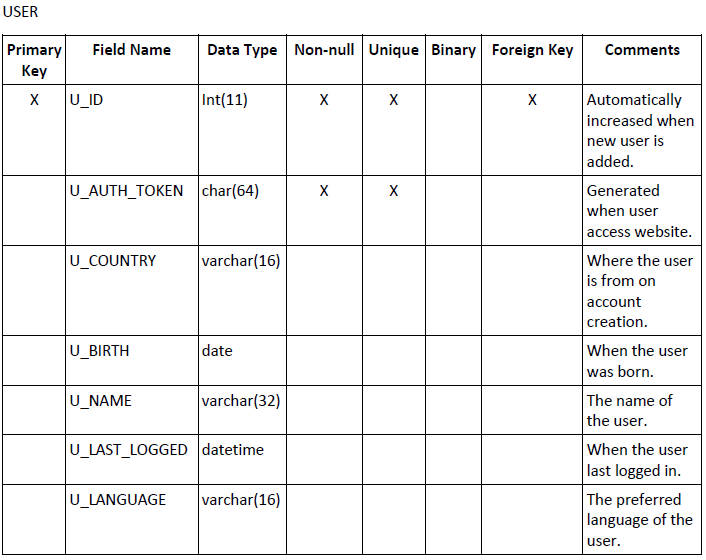
\includegraphics[scale=0.85,left]{er_tables/user.PNG}

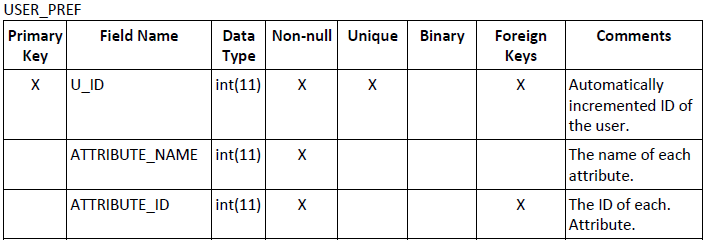
\includegraphics[scale=0.85,left]{er_tables/user_pref.PNG}

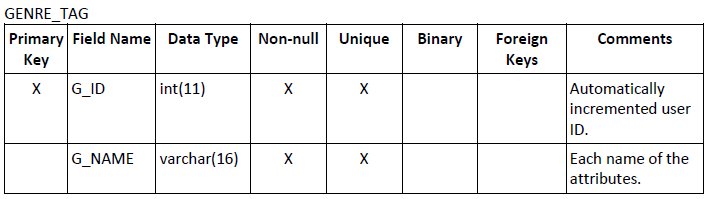
\includegraphics[scale=0.85,left]{er_tables/genre_tag.PNG}

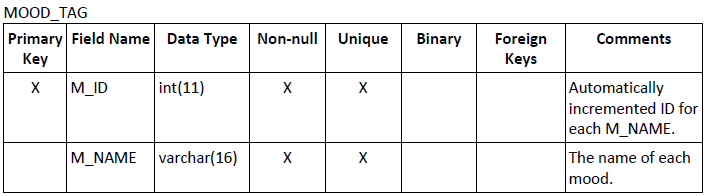
\includegraphics[scale=0.85,left]{er_tables/mood_tag.PNG}

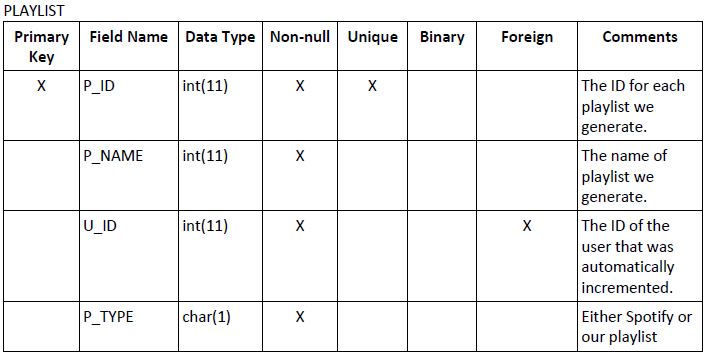
\includegraphics[scale=0.85,left]{er_tables/playlist.PNG}

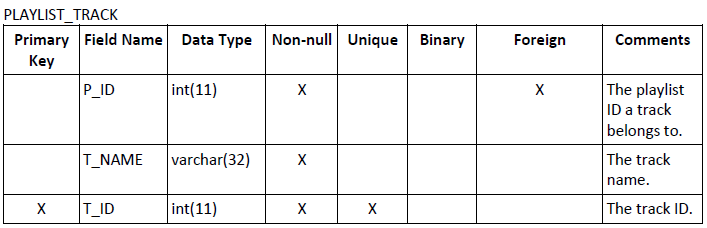
\includegraphics[scale=0.85,left]{er_tables/playlist_track.PNG}


\section*{System Architecture}

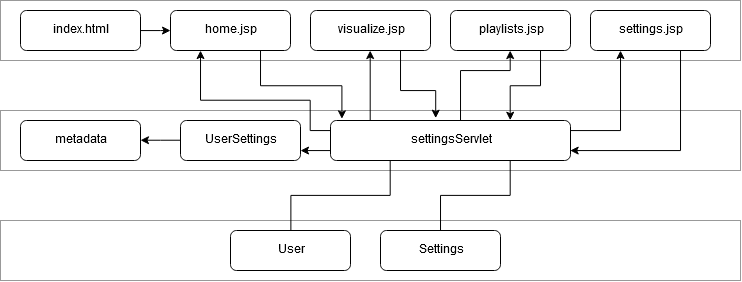
\includegraphics[scale=0.64,left]{er_tables/mvc.png}

The system architecture works as follows.
\begin{itemize}
    \item The user navigates to our website and is prompted by our logo and name of our website.
    \item All our Views include (home.jsp, visualize.jsp, playlists.jsp, settings.jsp).
    \item We have one controller that is called settingsServlet that has a class called UserSettings that holds all the attributes needed.
    \item Our model consists of (User, Settings).
    \item Upon signing into Spotify, the user is redirected to home.jsp.
    \item When the user wants to navigate to another page, the servlet or controller (settingsServlet) is used to navigate between pages and transfer any vital information a page is dependent on.
    \item Before Playlists.jsp can be populated with recommended content, the user must visit settings.jsp to save some preferences that they like. Once this happens, the controller will make a database query to store these user preferences.
    \item At any time, the user can update their preferences by revisiting the settings page and updating their updated preferences.
    \item Once this happens, playlists.jsp will utilize the preferences saved to recommend playlists from the information passed by the controller.
\end{itemize}

\section*{System Snapshot}
\begin{itemize}
    \item The user is first presented with our site, where they are given the option to try out the site using Spotify or try to use the site without using the music service. If choosing to connect with Spotify, they are redirected to a terms and conditions page, which will ask the user to grant permissions between our site and their account.
    
    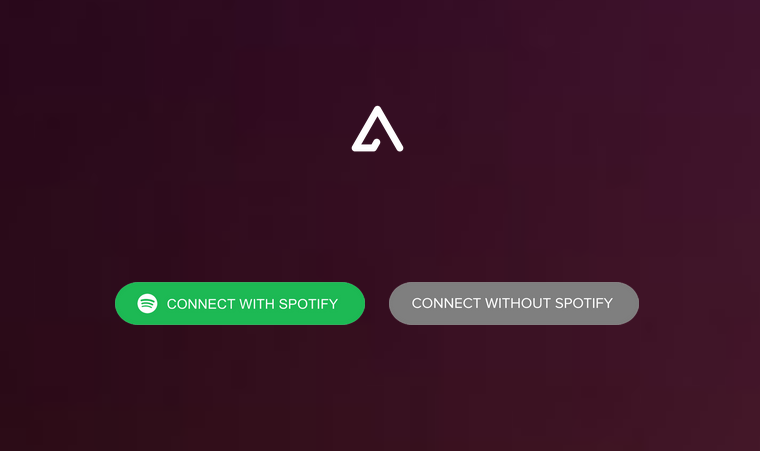
\includegraphics[scale=0.45,left]{snapshot/Capture.PNG}
    
    \item After logging in with the music streaming service, the user is redirected to the home page, which offers a few initial insights into what the site has to offer.
    
    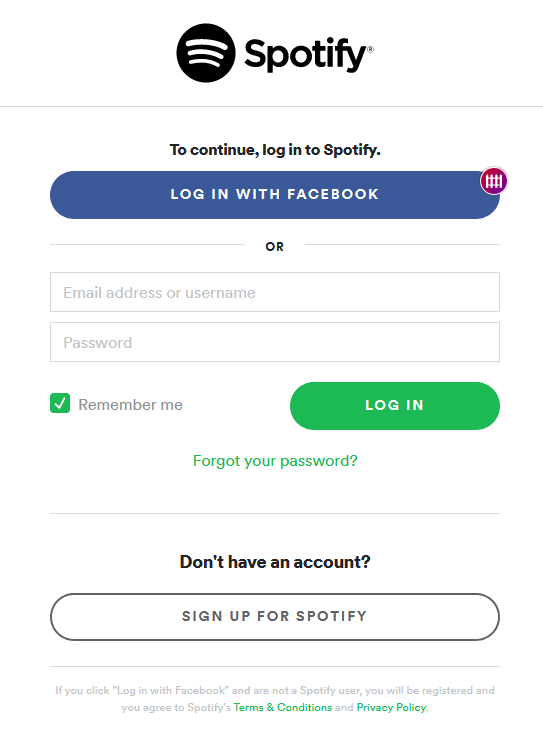
\includegraphics[scale=0.33,left]{snapshot/Capture8.PNG}
    
    \item Initially the user can see what the most recent track they listened was, within the last 24 hours. They are also able to visually see what how their listening habits are displayed visually. Beneath that is the last 5 tracks that have been listened to on the site.
    
    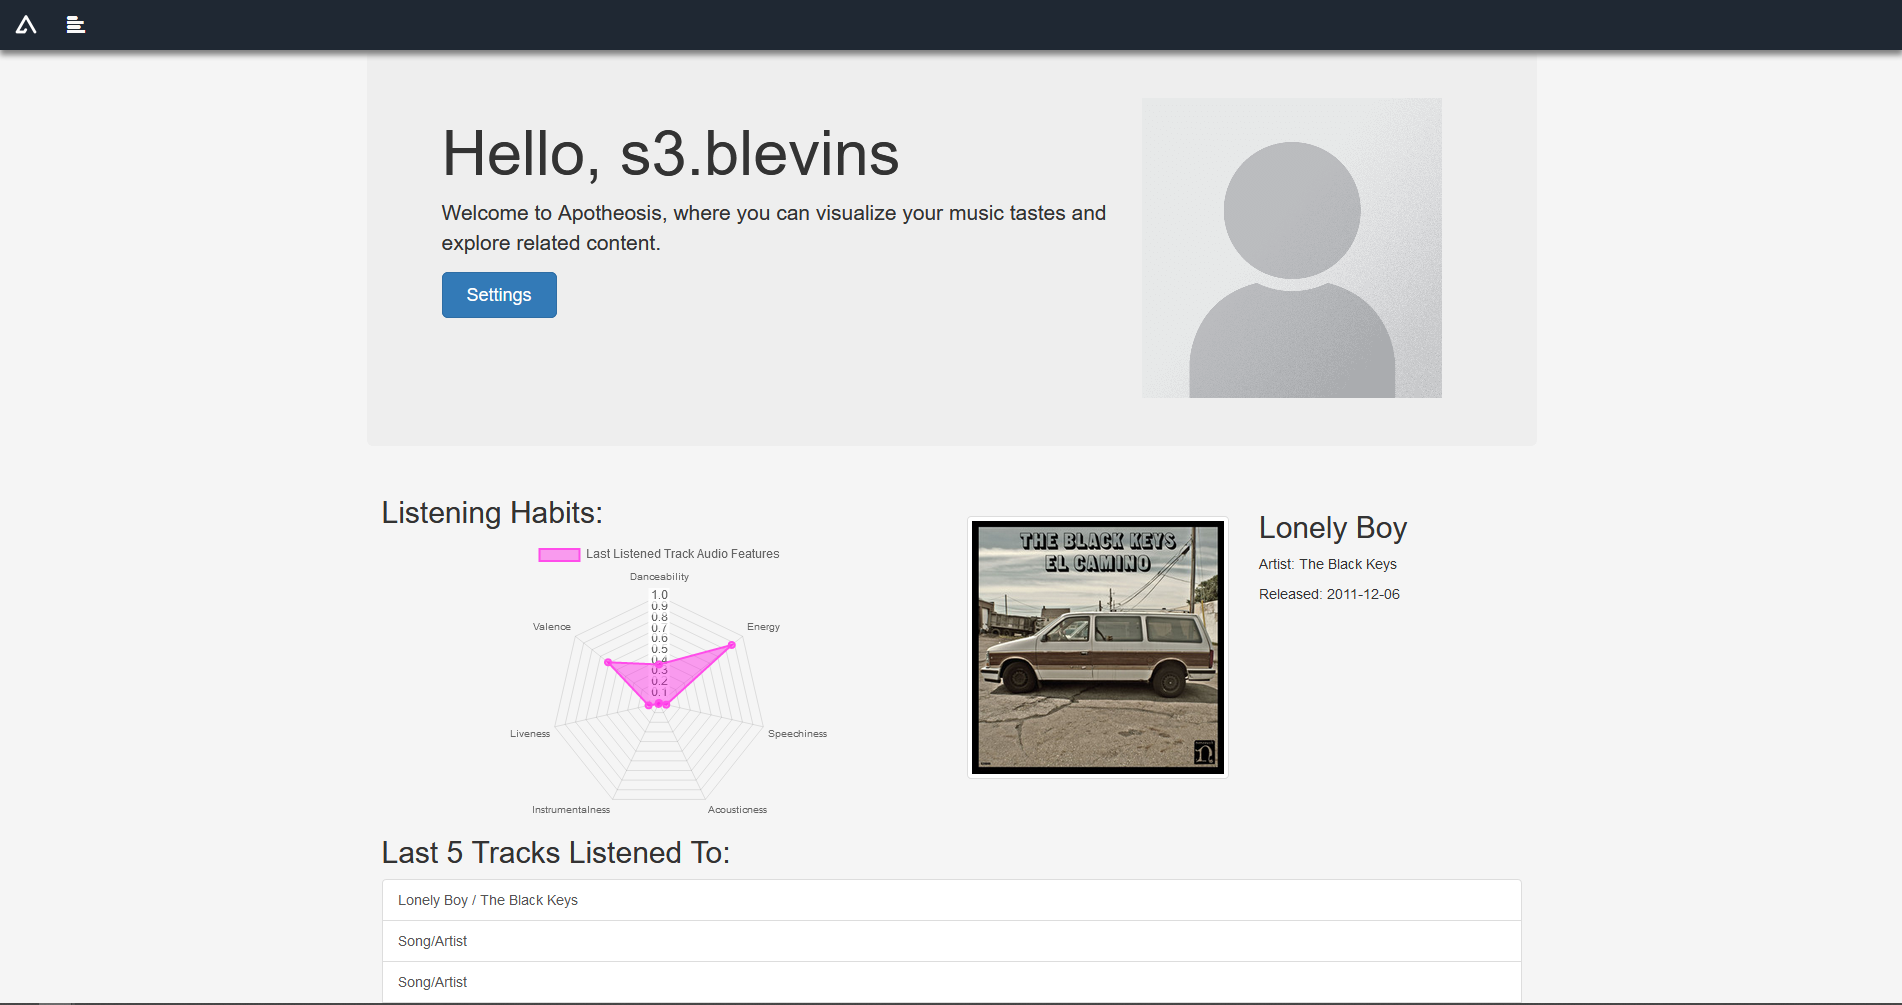
\includegraphics[scale=0.33,left]{snapshot/Capture1.PNG}
    
    \item Below that, the user can view the last saved tracks in their library, some statistics, along with a few music related facts.
    
    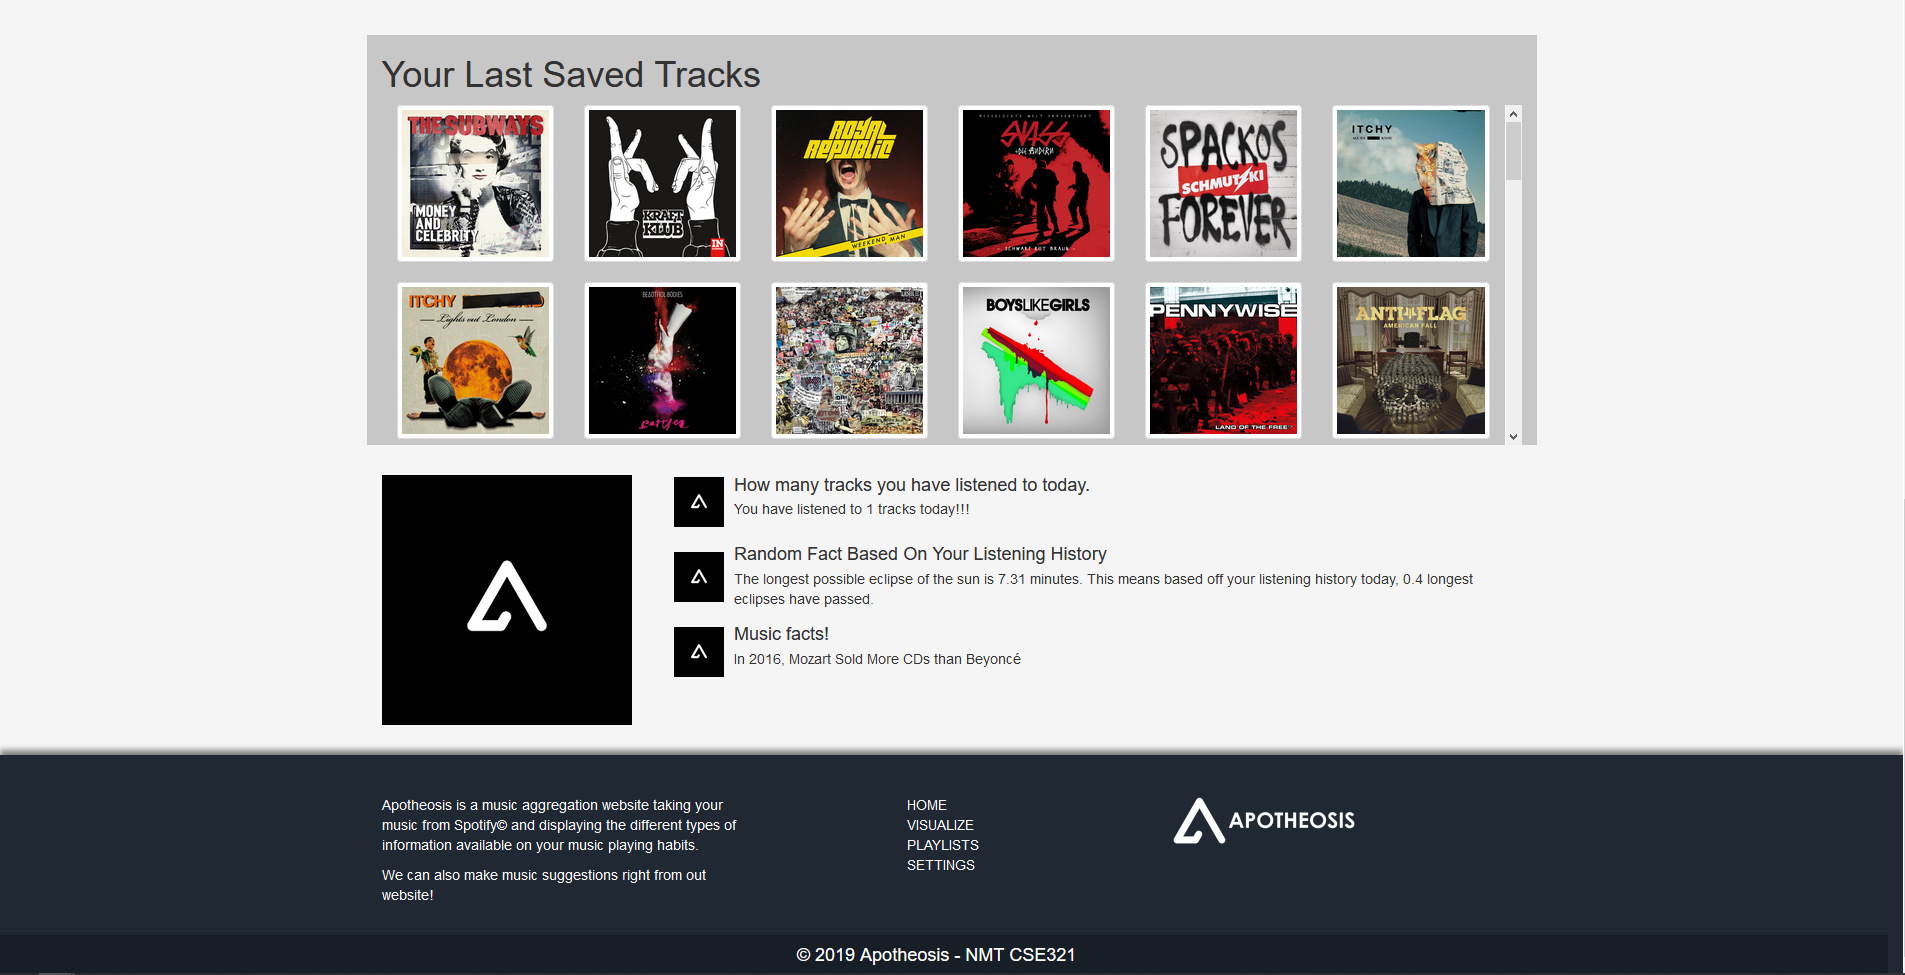
\includegraphics[scale=0.33,left]{snapshot/Capture2.PNG}
    
    \item Below that, the user can view the last saved tracks in their library, some statistics, along with a few music related facts.
    
    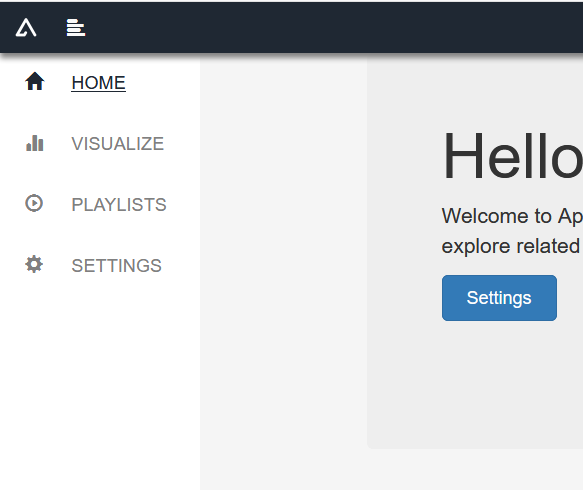
\includegraphics[scale=0.33,left]{snapshot/Capture3.PNG}
    
    \item The visualize page displays applicable information regarding the music and listening habits. It provides a view of recorded favorite genres, moods, styles and beats, and an analysis of your most listened to track.
    
    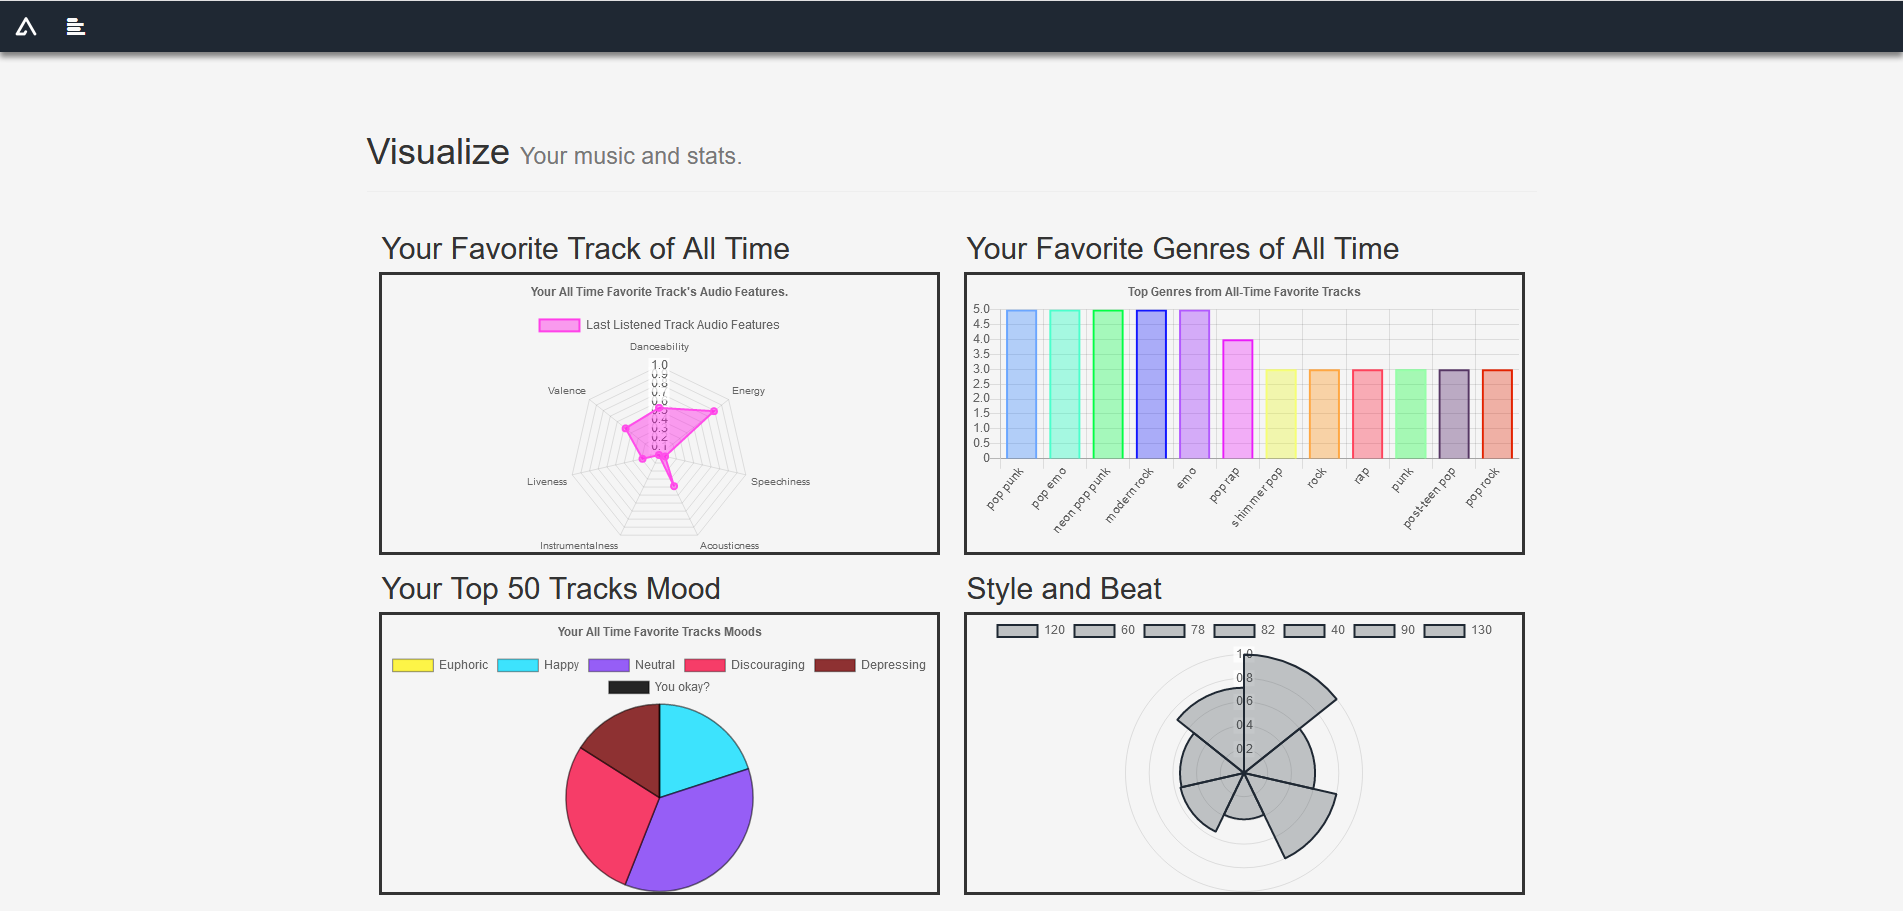
\includegraphics[scale=0.33,left]{snapshot/Capture4.PNG}
    
    \item The playlists page shows playlists created by Spotify, playlists made from our site's recommendations, in addition to artists based on those playlists, and popular playlists in your region.
    
    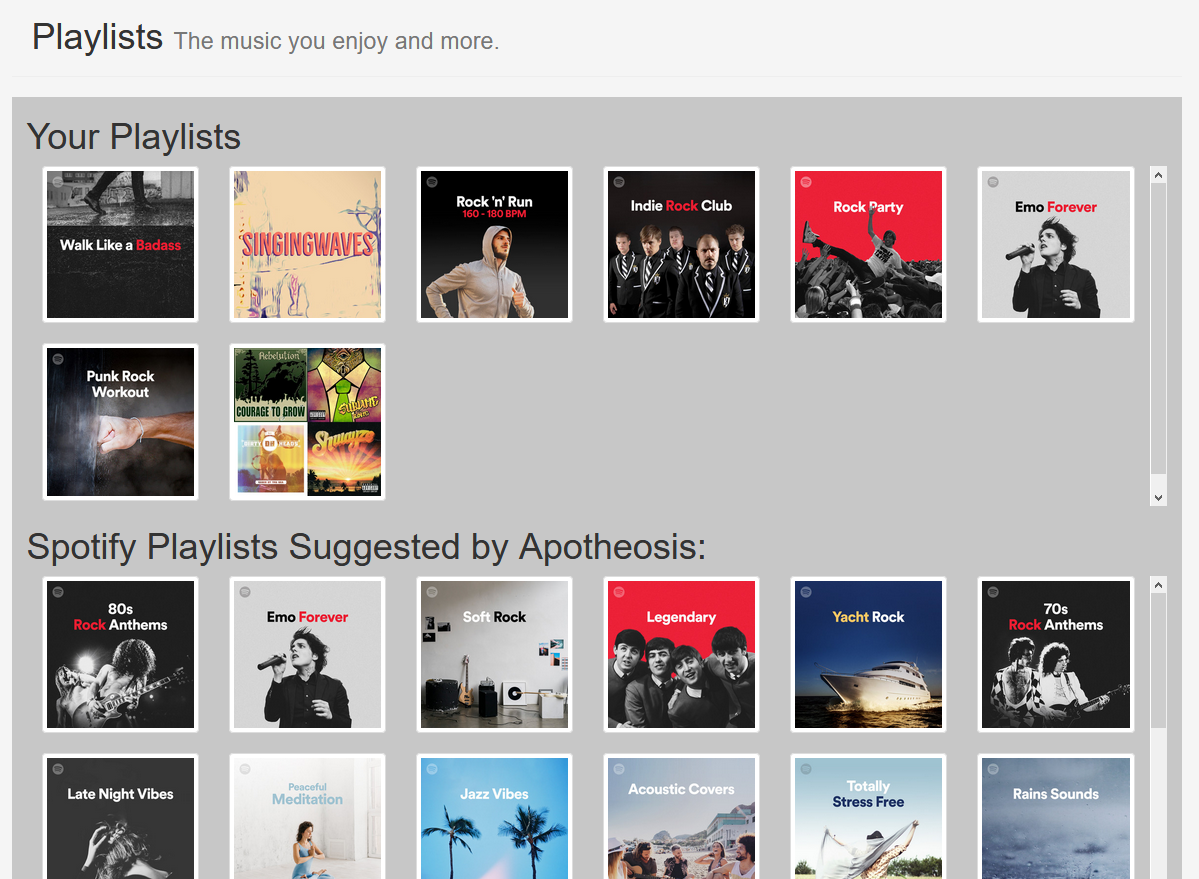
\includegraphics[scale=0.45,left]{snapshot/Capture6.PNG}
    
    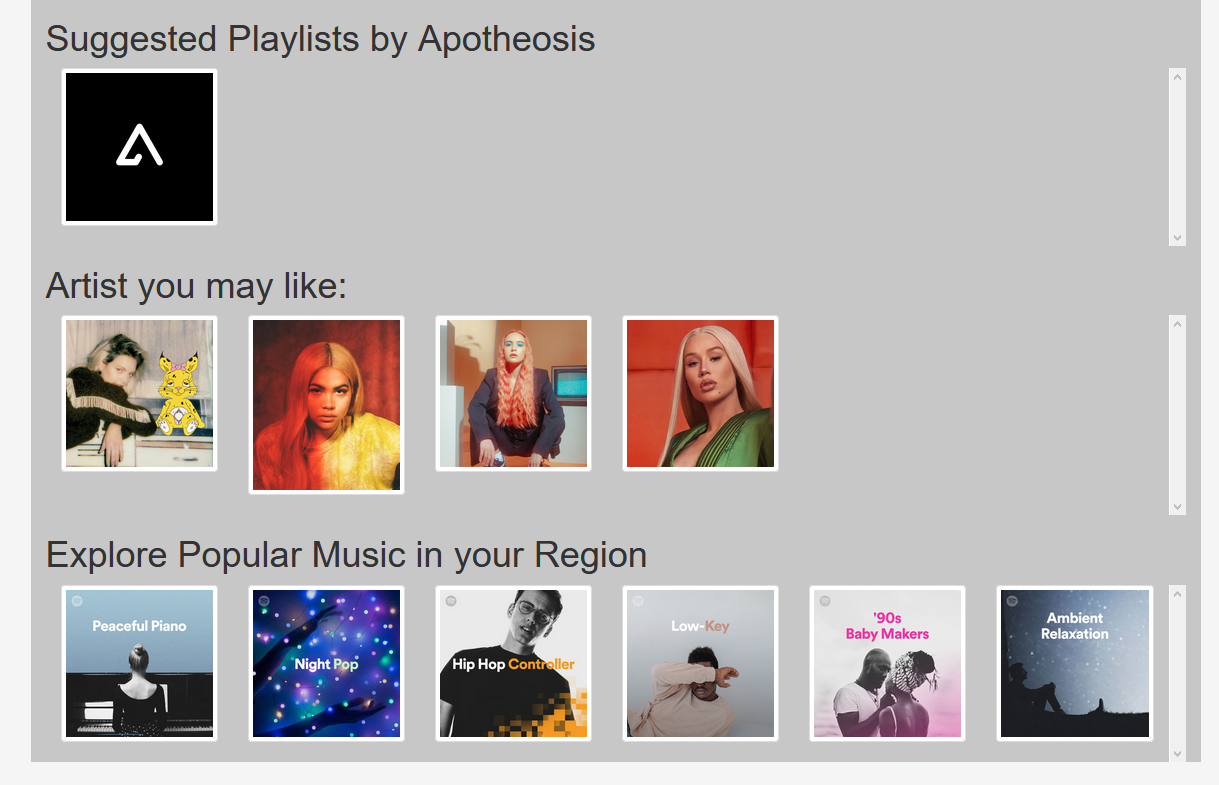
\includegraphics[scale=0.45,left]{snapshot/Capture7.PNG}
    
    \item Finally the settings page allows the user to enter their music preferences. The preferences are saved into the database, and the data is preserved based on the user's info. The settings are used to generate the playlists.
    
   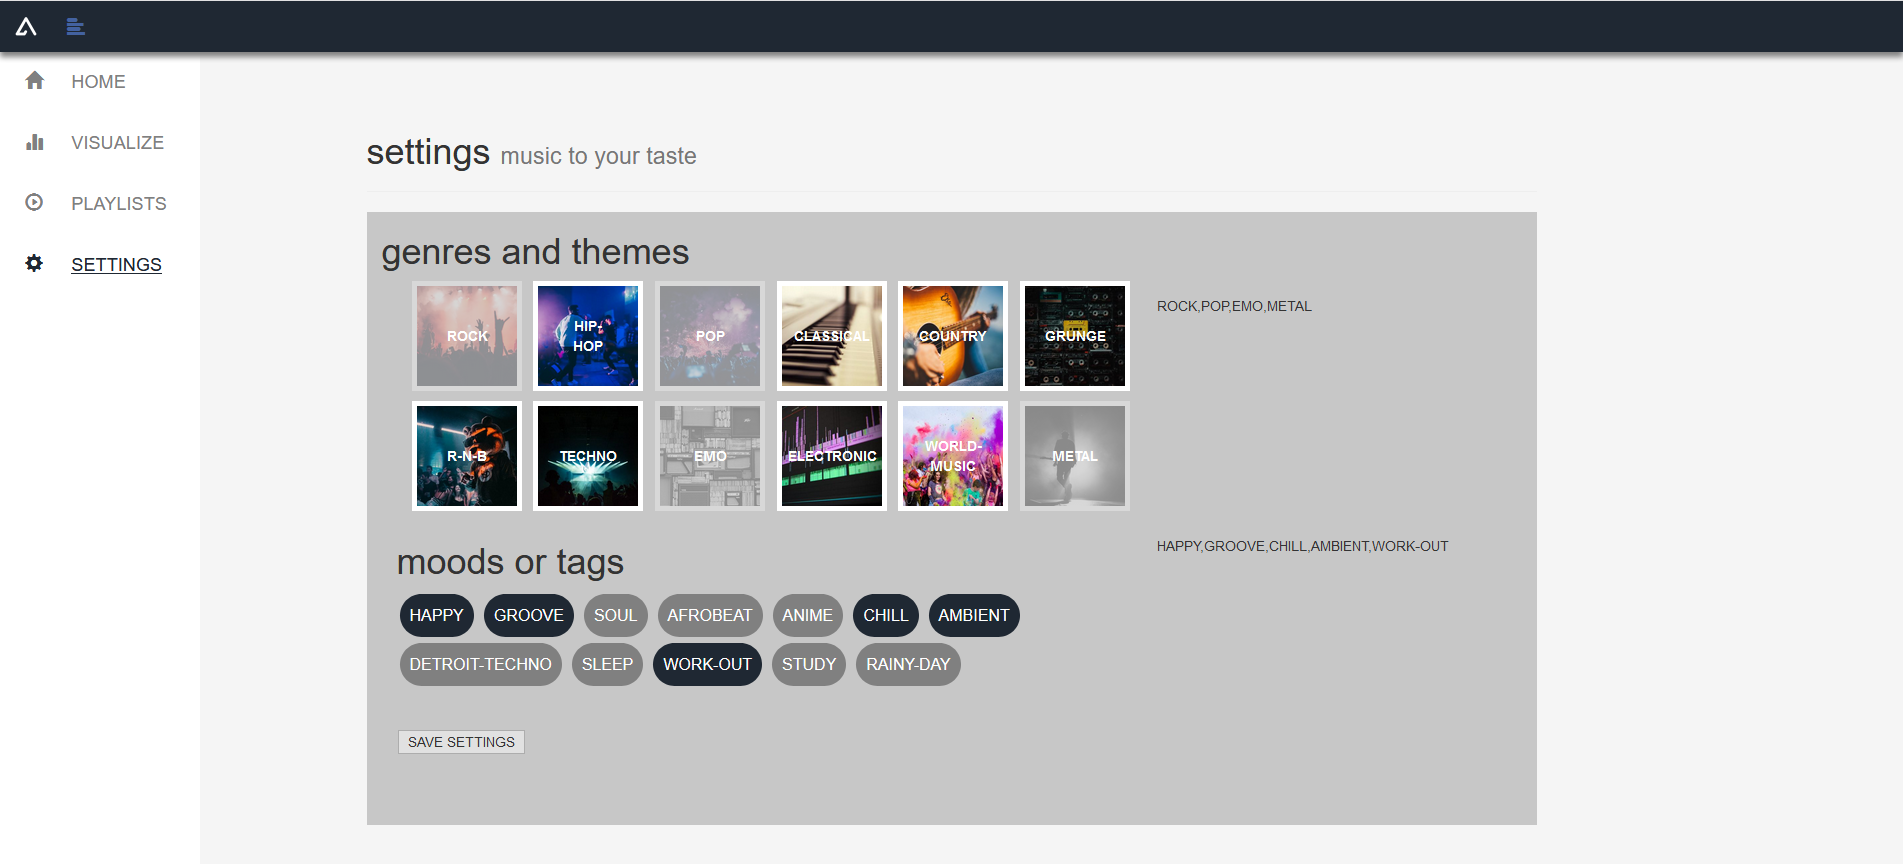
\includegraphics[scale=0.33,left]{snapshot/Capture5.PNG}
    
\end{itemize}


\section*{Conclusion}

What we have accomplish is as follows:
\begin{itemize}

    \item Preference saving of genres.
    \item Database interaction.
    \item MVC architecture.
    \item Recommended playlists based on preferences.
    \item Display statistics based on the user’s listening habits.
    \item Create our own interpretation of user listening and explain what aspects could mean for the user (i.e top 50 user track’s moods).
    \item Redirect users in a new tab to Spotify tracks, albums, or artists if they want to learn more about their music.
    \item Dynamic charts based on data using chart.js.
    \item A slide out menu that displays our pages we support.
    \item Follow User Authentication with OAuth 2.0.
    \item A site footer that explains what our website is about and the pages that a user can navigate.
\end{itemize}

Our project has accomplished the ability to store unique user’s preferences (genre liking) and utilizes this information to suggest likable playlists based on their interests in these genres. In addition, our project has adopted the Model, View, Controller (MVC) architecture. We have integrated views on our home page and visualize page to show user listening habits that range from their listening history, the last song they listened to audio features, their favorite genres, and much more to help them gain an understanding on how they listen and what it means.

Our project also allows our users the ability to investigate their saved artists, tracks, and listened to tracks to see what other information is tracked by Spotify.

For the future of this project, we would love to keep track of user information on a daily, weekly, monthly, and yearly basis to show them even more insights on their listening habits. We would also love to implement more random statistics and show them interesting and cool details (like our moon statistic on our website). In addition, we want to implement animations that would keep the user engaged and keep returning to our website (such as canvas videos that are available to select artists now). A cool feature we want to support in the future include synchronous LED playback which will light up an LED strip as the current music plays.  There are a few things that have not been implemented such as daily tracking of listening history that we would love to add in the future in addition to figuring out why on certain resolutions we have a padding above our page. Last, we would love to clean our code and organize it better to eventually make it open source and be an example for other developers to look at our source code as an example.



\section*{References}

\noindent
{\textsuperscript{[1]} https://musicaldata.com/} \\
{\textsuperscript{[2]} http://playlist-manager.com/} \\
{\textsuperscript{[3]} http://static.echonest.com/SpotifyPopcorn/}\\
{\textsuperscript{[4]} https://discoverquickly.com/}\\
{\textsuperscript{[5]} https://replayify.com/login}
\end{document}

